%%%%%%%%%%%%%%%%%%%%%%%%%%%%%%%%%%%%%%%%%%%%%%%%%%%%%%%%%%%%%%%%%%%%%%%%%%%%%%%%
%2345678901234567890123456789012345678901234567890123456789012345678901234567890
%        1         2         3         4         5         6         7         8

\documentclass[letterpaper, 10 pt, conference]{ieeeconf}  % Comment this line out
                                                          % if you need a4paper
%\documentclass[a4paper, 10pt, conference]{ieeeconf}      % Use this line for a4
                                                          % paper

\IEEEoverridecommandlockouts                              % This command is only
                                                          % needed if you want to
                                                          % use theplp \thanks command
\overrideIEEEmargins
% See the \addtolength command later in the file to balance the column lengths
% on the last page of the document



% The following packages can be found on http:\\www.ctan.org
\usepackage{graphics} % for pdf, bitmapped graphics files
\usepackage{epsfig} % for postscript graphics files
\usepackage{mathptmx} % assumes new font selection scheme installed
\usepackage{times} % assumes new font selection scheme installed
\usepackage{amsmath} % assumes amsmath package installed
\usepackage{amssymb}  % assumes amsmath package installed
\usepackage[noadjust]{cite}
\usepackage{dblfloatfix}
\usepackage{color}
\renewcommand{\thefigure}{\arabic{figure}}

\title{\LARGE \bf
Design of a Soft Wearable Elbow Exosuit for Lifting Assistance
}

%\author{ \parbox{3 in}{\centering Huibert Kwakernaak*
%         \thanks{*Use the $\backslash$thanks command to put information here}\\
%         Faculty of Electrical Engineering, Mathematics and Computer Science\\
%         University of Twente\\
%         7500 AE Enschede, The Netherlands\\
%         {\tt\small h.kwakernaak@autsubmit.com}}
%         \hspace*{ 0.5 in}
%         \parbox{3 in}{ \centering Pradeep Misra**
%         \thanks{**The footnote marks may be inserted manually}\\
%        Department of Electrical Engineering \\
%         Wright State University\\
%         Dayton, OH 45435, USA\\
%         {\tt\small pmisra@cs.wright.edu}}
%}

\author{Carly M. Thalman$^{1}$, \textit{Student Member, IEEE}, Quoc P. Lam$^{1}$, Pham H. Nguyen$^{1}$, \textit{Student Member, IEEE}, 
\\Saivimal Sridar$^{1}$, \textit{Student Member, IEEE}, and Panagiotis Polygerinos$^{1*}, \textit{Member, IEEE}$% <-this % stops a space
\thanks{*Corresponding Author}% <-this % stops a space
\thanks{$^{1}$ Carly M. Thalman, Quoc P. Lam, Pham H. Nguyen, Saivimal Sridar, and Panagiotis Polygerinos are with the Polytechnic School, Ira A. Fulton Schools of Engineering, Arizona State University, Mesa, AZ 85212, USA.
        {\tt\small cmthalma@asu.edu, qlam1@asu.edu, nhpham2@asu.edu, ssridar@asu.edu, polygerinos@asu.edu}}%
}


\begin{document}



\maketitle
\thispagestyle{empty}
\pagestyle{empty}


%%%%%%%%%%%%%%%%%%%%%%%%%%%%%%%%%%%%%%%%%%%%%%%%%%%%%%%%%%%%%%%%%%%%%%%%%%%%%%%%
\begin{abstract}

The soft robotic brace provides ergonomic lifting assistance to industrial warehouse workers who put a significant amount of strain on their elbow joints due to repetitive lifting. The brace consists of a novel array of soft, pneumatically controlled actuators that, when inflated, conform around the elbow joint and provide elbow flexion assistance.  The exosuit actuators were shown to reveal extremely high force-to-weight ratios and the exosuit was predicted to aimed to achieve up to 30 Nm of torque to support the user’s elbow.  The efficacy of the exosuit design underwent participant testing and was shown to provide assistance to the user bearing various loads with the elbow at a 90 degree bend, while decreasing muscle activity in the bicep and keeping most of the user's natural range of motion.



\end{abstract}


%%%%%%%%%%%%%%%%%%%%%%%%%%%%%%%%%%%%%%%%%%%%%%%%%%%%%%%%%%%%%%%%%%%%%%%%%%%%%%%%
\section{INTRODUCTION}

Freight, stock, and warehouse workers are required to perform strenuous and repetitive tasks like packing, shelving, loading, and unloading goods on a daily basis. These repetitive motions can lead to fatiguing, that reduces productivity, as well as lower-back and upper-limb injuries. Injuries in this line of work are generally musculoskeletal disorders (MSDs) that can be caused by improper lifting postures, repetitive high strain activities, and age-related factors \cite{BLS2017}. 

According to the US Department of Labor in 2015, there were 376,190 cases (33\% of all injury cases) of MSDs caused by overexertion in lifting \cite{BLS2016}. Of all the occupations, laborers and freight, stock, and material movers were part of the highest number of injury cases in 2015 \cite{BLS2016}. The cost of workplace injury in the USA amounted to be around \$190 billion and has resulted in over 1.1 million lost days of work \cite{Leigh2011}. There has also been a consistent increase in the age of the labor force since the beginning of the century (the median age is around 48 years old) and the 45 and over category of workers have grown from 34\% to 44\% of the total labor force, since 2000 \cite{Mislinski2017}. Therefore, there is a need to assist aging laborers and freight, stock, and material movers to perform these arduous tasks in order to reduce fatigue to improve task efficiency and the health of these workers. 

\begin{figure}[t!]
\centering
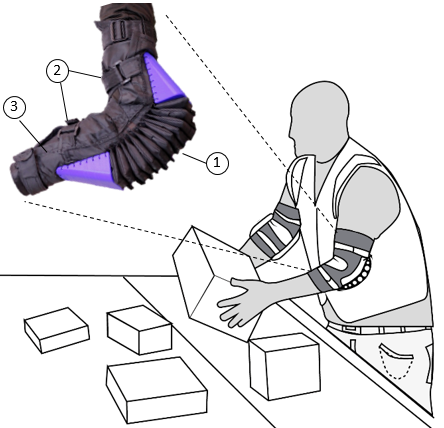
\includegraphics[width=0.5\textwidth]{Concept.PNG}
\caption{(Illustration of the concept of the soft wearable exosuit for lifting assistance in warehouse environment. Key design elements include: (1) Straps to tighten and loosen the exosuit. (2) Network of actuators for flexion motion of elbow.  (3) Elastic elbow-sleeve to attach exosuit to user’s arm. (4) Two pockets of actuators for extension motion of elbow. (5) Conveyor Belt carrying boxes of goods for transportation.}
\label{fig:concept}
\end{figure}

According to the US Department of Labor in 2015, there were 376,190 cases (33\% of all injury cases) of MSDs caused by overexertion in lifting \cite{BLS2016}. Of all the occupations, laborers and freight, stock, and material movers were part of the highest number of injury cases in 2015 \cite{BLS2016}. The cost of workplace injury in the USA amounted to be around \$190 billion and has resulted in over 1.1 million lost days of work \cite{Leigh2011}. There has also been a consistent increase in the age of the labor force since the beginning of the century (the median age is around 48 years old) and the 45 and over category of workers have grown from 34\% to 44\% of the total labor force, since 2000 \cite{Mislinski2017}. Therefore, there is a need to assist aging laborers and freight, stock, and material movers to perform these arduous tasks in order to reduce fatigue to improve task efficiency and the health of these workers. 

Potential solutions for approaching this problem have been seen in the field of wearable robotics and human augmentation. Human augmentation robotic devices are designed to help augment load carriage capacity and normal muscle function in healthy individuals while reducing the amount of physical exertion the user is required to sustain. Examples of human augmentation via exoskeletons have been seen for multi-purposes in healthcare, rehabilitation, and industrial settings \cite{Kazerooni2008}. There have been a variety of lower-limb exoskeletons \cite{Viteckova2013} and upper-limb devices \cite{Gopura2016}. These devices look to increase the load bearing capability of the user. The primary concerns of using exoskeletons is its rigidity, high cost, portability, alignment complications with the biological joint it is trying to assist, and finally the comfort over long periods of use.

The recent introduction and advancement of soft robotics has led to promising designs of wearable devices that are compliant, safe for human-robot interaction, lightweight, low-cost to fabricate, allows even distribution of force on the users joints, and are unaffected by alignment issues like with rigid exoskeletons \cite{ADEM:ADEM201700016}. These intrinsically soft wearable devices have been categorized based on their novel form of actuation, including cable-driven actuators \cite{Gopura2016,Dinh2017,Xiloyannis2017,Ding2017}, pneumatic artificial muscles\cite{Park2014c,CALDWELL2007,Al-fahaam2017}, fluidic elastomeric actuators\cite{Polygerinos,Koh2017,Chen2017h}, and pneumatically inflatable bladder-based actuators \cite{Kim2017,Sridar2017,Simpson2017,Koh2017}.

\section{DESIGN OF THE SOFT ELBOW SUIT}
The functional requirements of the device are listed in Table X.  The major functional requirement set for the soft elbow brace was the overall force and torque output of the device,  at the worst-case scenario of a 90 degree bend in the elbow.  The natural range of motion for the elbow joint is a 135 degree bend, and no to prevent the device from hindering motion it must be able to allow the user to bend their arm at least 90\% of this range.  The device also should not exceed the combined weight of the average human forearm and hand at 2.3kg.

\begin{figure}[t!]
\centering
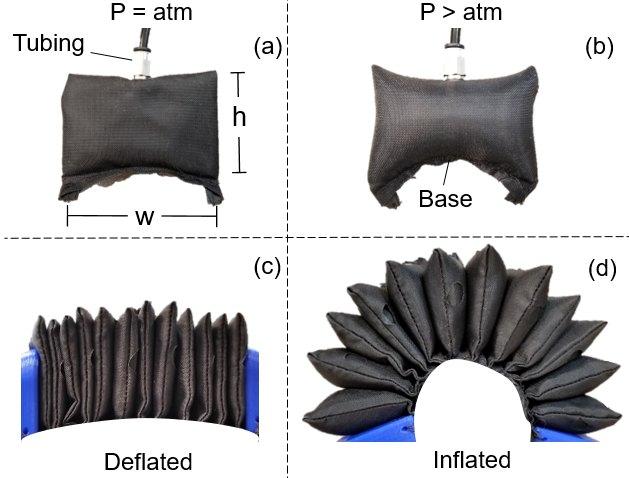
\includegraphics[width=0.3\textwidth]{V1_device.PNG}
\caption{(THIS WILL BE UPDATED WITH NEW DEVICE PIC) User wearing the Soft Robotic Elbow Suit (left) and the Elbow suit mounted to the test arm/elbow joint (right)}
\label{fig:user}
\end{figure}


\subsection{Functional Requirements and Design Considerations}
The design of the proposed soft elbow exosuit is aimed at providing assistance during activities involving bicep contraction, such as lifting and manipulating heavy objects within an industrial setting. Workers are often met with long shifts that would necessitate maximum comfort for extended periods of use, therefore soft compliant materials were selected as the material of choice. Ergonomics are also taken into consideration where the goal is to create a low-profile design that does not limit the user’s range of motion (ROM). 

To avoid obstructing the user's movement, the actuator design uses an array of hermetically sealed, and nylon encased bladders proximally mounted to the backside of the elbow joint. The individual bladders are created by heat sealing the borders of two rectangular layers of thermoplastic polyurethane (TPU) (DT-2001, American Polyfilms, Branford, CT) cut on a CNC laser cutter (MODEL, MAKE, LOCATION) and  with a modified soldering iron for the complex curvature of the base seal, and finished with an impulse sealer (model make location) once internal fittings had been attached. As the sealed bladder is inflated, the rectangular section forms a cylindrical shape. The a TPU bladder on its own is capable of supporting moderate pressures before risk of bursting or permanent deformation. However, by encasing the bladders in an inextensible, weaved nylon material (model make location) of the same net shape, higher actuation pressures can be utilized, therefore, generating a much higher stiffness when over pressurized. 

Research has shown that the average male, aged 23 +/- 2 years (check numbers) is capable of producing an average of 60 Nm of torque, at a 90 degree bend, during maximum voluntary muscle contraction [“Maximum elbow joint torques for digital human models”]. This is approximately 200 N (45 lbf) per arm, and in total, twice the industry’s safety standard for individual lifting capacity {CITATION}. In the average female, however, this torque values falls to 34Nm at maximum, which is much closer to the industry standard [“DESIGN OF APPARATUS TO STUDY HUMAN ELBOW JOINT MOTION”]. Assuming all lifting is done by the bicep, the goal of the soft elbow exosuit is to generate 30 Nm of torque at to supplement the user’s lifting capacity for a safe industry standard for lifting.


\begin{figure}[t!]
\centering
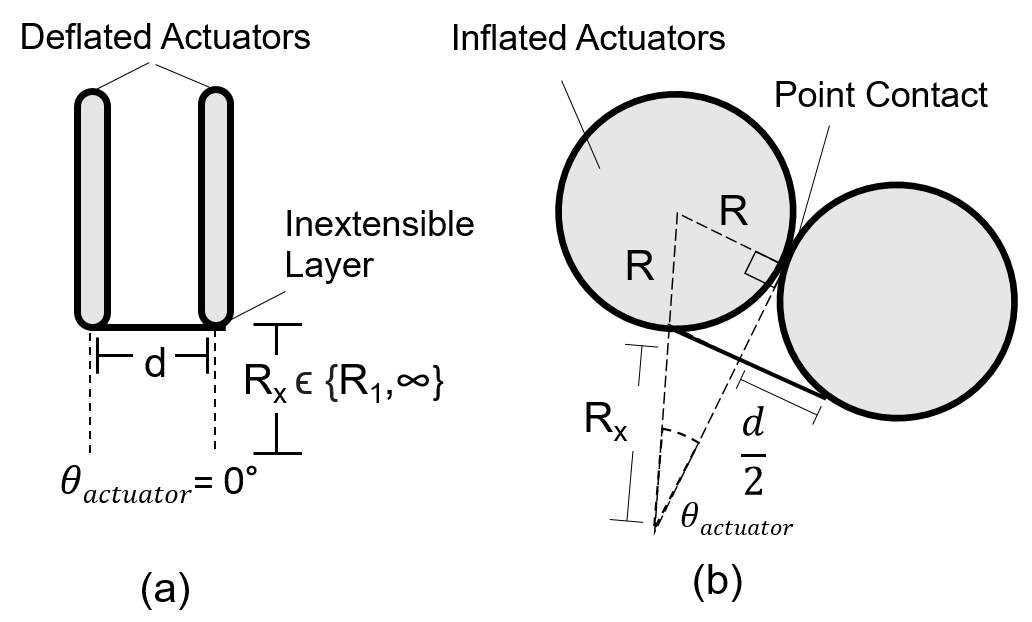
\includegraphics[width=0.4\textwidth]{ActuatorModel1.PNG}
\caption{Geometric analytical model of actuator behavior patterns in varying configurations of sizes}
\label{fig:Model1}
\end{figure}

\subsubsection{Extension Actuators}
PLACEHOLDER - Discuss with Panos???

\subsubsection{Flexion Actuator}
The flexion actuator utilized in the elbow suit was designed to provide a torque of 30 \textit{Nm} about the elbow joint to provide assistance to the bicep muscles. The proposed method involves Using a linear array of smaller cylindrical bladders anchored in equidistant positions about the axis of rotation (elbow joint) where a model of torque generation can be determined using simple geometry of the surfaces in contact. 

\subsection{Modeling of Actuators}
The starting point of selecting the range of design parameters was modeled based on first finding a way to maximize bending angle (SHOW FIGURES). Due to physical limitation of this specific manufacturing process, the distance must be at least 5mm, and the possible angles have been limited to 90 degrees, as an angle greater than this would not be realistic to assume between the two cylinders.  

\begin{equation}\label{eq. X15}
	\theta=sin^{-1}(1-d/r) 
\end{equation}
\begin{equation}\label{eq. X15}
	r > d 
\end{equation}


Using Equation (1) as a guideline and adding feasibility criteria for the dimensions, the \textit{distance} and \textit{radius} for the flexion actuator were determined with a combination of the two graphs shown in figure X. The flexion actuator was designed for a bending of 145$^{\circ}$. A suitable width of 75mm was selected for the actuator based on the available area behind the arm. The individual actuators were fabricated by heat sealing TPU to comply with the aforementioned dimensions. The actuators were encapsulated in nylon to withstand higher pressures in turn providing larger bending moment.  Section X showcases the higher operating pressures and forces that can be generate by this actuator design.  It is also assumed that the angle between pleats will never reach 90 degrees, as this would set the pleats perpendicular to one another which is not realistically feasible in the application of this device.  

The equation derived for theta in Fig. X above was then plotted for various radius and distance values to begin to observe the behavior of the more simplistic model and allow for easier selection of the design criteria used in following force and torque models.  The plot of the left shows the behavior of the interaction of two bladders when the radius is increased for various fixed distances.  As the radius increases, so does the bending angle for each fixed distance between the actuators.  The second plot shows the same information, but this time plotted with increasing distance at various fixed radii.  This relationship illustrates that as the distance between pleats increases, the bending angle decreases.  For all cases above, it is assumed that the radius is always larger than the distance in every case, and the boundary condition denoted in the red region is all cases in which the distance is below the limitation of 5mm set by the specific fabrication process used. 

\begin{figure}[t!]
\centering
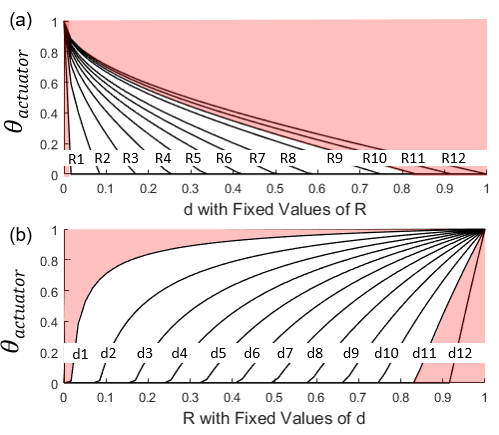
\includegraphics[width=0.5\textwidth]{graphs_model1.PNG}
\caption{This model assumes that each bladder has reached a steady-state pressure and will not deform during bending.  It is also assumed that each bladder will inflate to form a perfect circle.  (a) shows the relationship between bending angle and a changing actuator radius given a fixed distance between each bladder.  (b) shows the relationship between bending angle and a changing distance given a fixed radius.}
\label{fig:Graphs1}
\end{figure}	
\section{Analytical Modeling}

Modeling torque generation of the actuators follows the same geometric principles outlined in calculating bending angle. Line contact is replaced with the interacting area of each actuator, and as a result, pressure can be directly correlated with force output and therefore torque. Since geometry of the bladder array is identical across its width, two-dimensional representation of the interacting bladder is possible to simplify the mathematical model (Fig. xx.). 

\begin{figure}[t!]
\centering
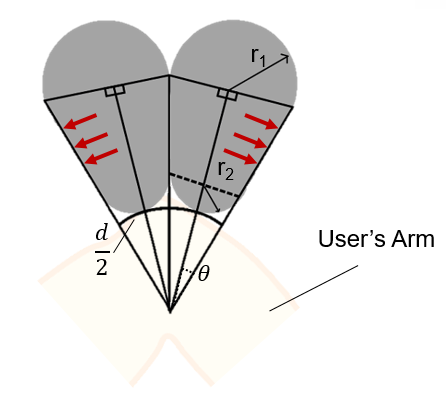
\includegraphics[width=0.3\textwidth]{model1.PNG}
\caption{View of two interacting bladders placed in an enlarged/exaggerated method along the outside of a user’s arm to demonstrate the overall placement}
\label{fig:mod1}
\end{figure}

Some basic assumptions are used in the model. < this will be written in paragraph form.
Bladder spacing is equidistant
Radius of elbow joint is spherical with radius 37 \textit{mm}
Bladder shape is rectangular 
Unconstrained boundaries of the bladders above and below the area of contact form semi-circles
Bending angle is related to center of curvature of the bladder base by the relationship 
(insert eq.) 
The centerline of each individual bladder converges at the center of curvature

	As bending angle of the arm ranges from zero to a human average range-of-motion  of $135^o$, the length of the actuator will bend to produce the same angle where its arc length, S remains constant, defined by Eq. X2. As a result of equidistant spacing of the bladders, the radius of the arc length’s curvature, $R_x$ must therefore vary from ${\inf}$ to $R_{1}$, where $R_x$ is inversely dependent on bending angle,  $\Theta_0$ (Eq. X3).
 
\begin{equation}
	S = R_1\theta_{max}
\end{equation}
\begin{equation}
	R_x(\theta_0) = R_1\frac{\theta_{max}}{\theta_0}
\end{equation}

Given the geometrical relationships in equation 2 and 3, length of interaction, L can be defined by the resulting geometry of the interacting bladders where a half section is depicted in figure X. Since bladder circumference remains constant, the equation

\begin{equation}\label{eq. X4}
	\pi R = L + \frac{\pi}{2}(r_1+r_2)
\end{equation}

can be used to find L. Solving for the inner and outer radius, $r_1$ and $r_2$, respectively, requires additional trigonometric relations, where


\begin{figure}[t!]
\centering
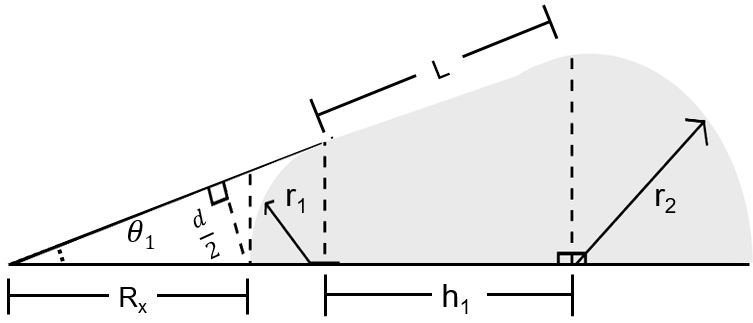
\includegraphics[width=0.5\textwidth]{model2.PNG}
\caption{View of two interacting bladders placed in an enlarged/exaggerated method along the outside of a user’s arm to demonstrate the overall placement}
\label{fig:mod1}
\end{figure}

\begin{figure}[t!]
\centering
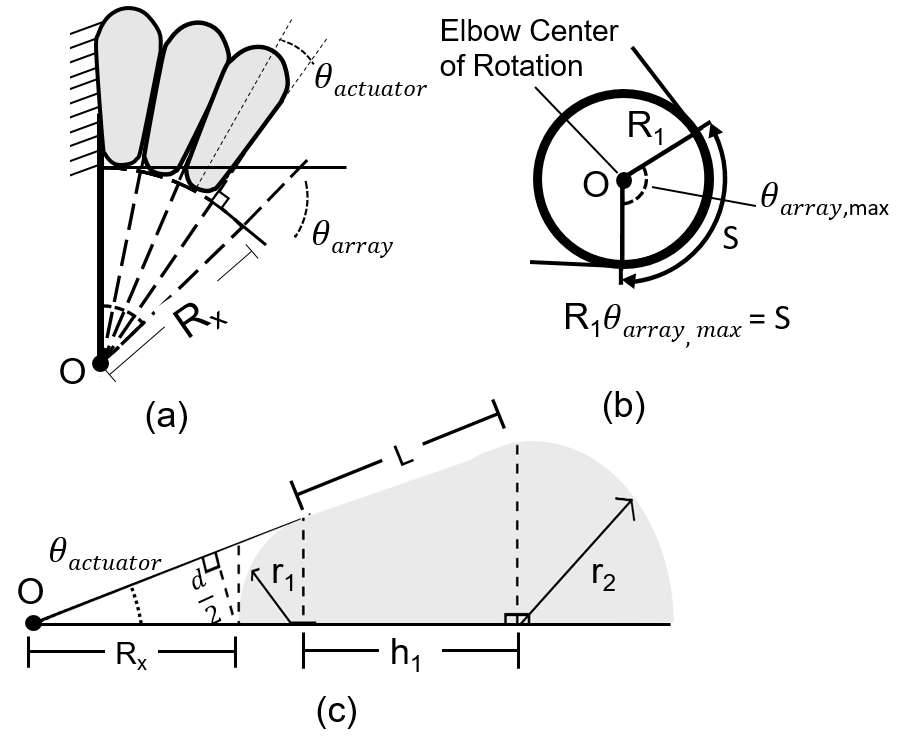
\includegraphics[width=0.5\textwidth]{model3.PNG}
\caption{View of two interacting bladders placed in an enlarged/exaggerated method along the outside of a user’s arm to demonstrate the overall placement}
\label{fig:mod1}
\end{figure}

\begin{equation}\label{eq. X5}
	tan(\theta_0) = \frac{r_1}{R_x+r_1} = \frac{d}{2R_xcos(\theta_0)}
\end{equation}
And
\begin{equation}\label{eq. X6}
	tan(\theta_0) = \frac{r_2}{R_x+r_1+L_1} = \frac{r_1}{R_x+r_1}
\end{equation}

Solving for $r_1$ is straightforward using algebraic manipulation, resulting in 
\begin{equation}
	r_1(\theta_1)  = \frac{dR_x}{2R_xcos(\frac{\theta_0}{2\textit{n}})},
\end{equation}
whereas solving for $r_2$ requires additional substitutions and a quadratic solution to the second order polynomial,

\begin{equation}\label{eq. X7}
	ar_2^2+br_2-c = 0,
\end{equation}

With,

\begin{equation}\label{eq. X8}
	a = 1+\frac{1}{\tau}+(\frac{\pi}{2})^2
\end{equation}
\begin{equation}\label{eq. X9}
	b = \pi^2R+\pi\lambda-\frac{\pi^2r_1}{2}
\end{equation}
\begin{equation}\label{eq. X10}
	c = (\pi R+\lambda)^2- stuff
\end{equation}

Additional substitutions for groups of parameters are as followed,

\begin{equation}\label{eq. X11}
	\alpha = (\pi R+\lambda)^2
\end{equation}
\begin{equation}\label{eq. X12}
	\beta = -\pi^2Rr_1+(\frac{\pi R}{2})^2-\lambda\pi r_1
\end{equation}
\begin{equation}\label{eq. X13}
	\lambda = \sqrt{(R_x+r_q)^2+r_1^2}
\end{equation}
\begin{equation}\label{eq. X14}
	\tau = (\frac{r_1}{R_x+r_1})^2
\end{equation}

Using length of interaction, L, the effective force can be calculated to determine the torque it would generate about the elbow joint. Since Pressure, P is equal at every point in pneumatic systems, force, F is also distributed evenly across the interacting area (LW) and is represented as a point load applied at a distance of 

\begin{equation}
	L_f = 
\end{equation}

away from the elbow’s axis of rotation and parallel to the direction of the arm. 

Loop functions were created inside MATLAB to generate torque values for various inputs, i.e. bladder heights, quantity of bladders and bending angles (Fig. XX). These were the three main considerations for inputs based on design constraints in which the remaining parameters are directly derived from them. Pressure input was set to a reasonable limit of 300kPa where torque has a linear dependency on pressure as shown in Eq. 16, therefore only one set pressure was modeled for. 

\begin{equation}\label{eq. X16}
	T = F L_f      ;     F = \frac{P}{LW} 
\end{equation}

\begin{table}[h]
\caption{Final Design Parameters Selected
}
\label{Functional Requirements}
\begin{center}
\renewcommand{\arraystretch}{1.5} % Default value: 1
\begin{tabular}{| c | c | c | c |}
\hline
\textbf{Distance} & \textbf{Height}  & \textbf{Width} & \textbf{Number}\\ 

\hline

8mm &  44mm  & 75mm & 12 Pleats\\ 

\hline

\end{tabular}
\end{center}
\end{table}

\section{Device Fabrication}

\begin{figure}[t!]
\centering
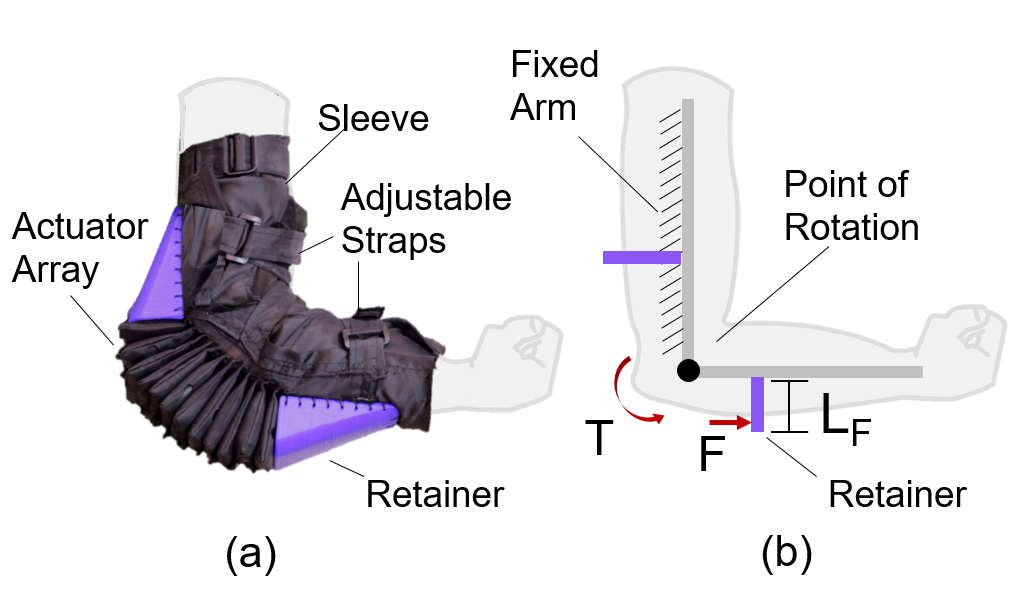
\includegraphics[width=0.5\textwidth]{arm.PNG}
\caption{Final Design of the soft robotic elbow sleeve (left) worn by a user, and the basic torque model concept behind the device (right)}
\label{fig:stifftest}
\end{figure}

\begin{figure}[t!]
\centering
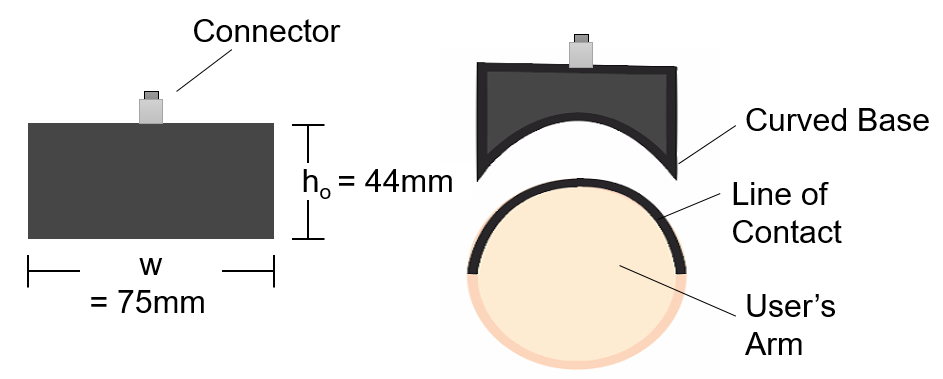
\includegraphics[width=0.3\textwidth]{bladders.PNG}
\caption{Cross-section of the user’s arm showing a side view of a single actuator (left), and a single actuator from the side view showing the curvature of the base (right).}
\label{fig:stifftest}
\end{figure}


The above force and torque models assume that the inflating actuators are always perpendicular to the arm at the point that each one is fixed.  However, in reality, when mounted on the arm the device does not behave in this way, as the forces generated between each bladder cause the adjacent bladders to fold over and bend freely until completely collapsed.  This causes a major loss in the forces generated the moment about the arm.  As a solution, end-stop bladders were designed and fixed to each end of the array of bladders to prevent the last bladders in the array from collapsing against the body.

These end-stops show shown in figure X provide the last step of the moment arm which was predicted to output the expected torque values from the design.  It is because of this moment arm that the device is as effective as shown in the models.  


The design of each individual actuator has an added line of curvature along the base.  This is to ensure that the flexion actuator maintains a continuous line of contact along the curvature of the arm, rather than the line contact a perfectly cylindrical shaped actuator would have when inflated against the contours of the arm.  This is to help prevent lifting, as well as to help distribute the forces along the entire contact area with the arm and the actuators. 

The nylon fabric and TPU was cut using a precision laser cutter to ensure the dimensions were accurate.  Metal push-to-connect fittings were then placed on the top of each bladder to allow for tubing to connect for pressurization.  Placing the fittings on the top as shown in figure X allows for the bladders to fully expand without interfering with point of connection.


\section{Testing of Device}

\subsection{Stiffness Test of Single Actuator}

A single \textcolor{red}{bladder} was tested for durability and strength.  To showcase the ability of this actuator design, a single bladder was placed in a uniaxial tensile strength machine and fixed between two plates fixed 8mm apart - the same distance fixed between actuators in the array.  The actuator was then inflated in increments of 20kPa up to 300kPa.  This test resulted in a linear relationship between the force generated by a single actuator and the pressure used to inflate it, as well as a average maximum force of 567.8 N with a standard deviation of 3. 56 for a total of 5 total tests on the single bladder.  Next, to test the stiffness of the device, it was inflated to the maximum tested pressure of 300kPa and then placed between the two plates.  Using the same force measured in the first test as a threshold, the bladder was displaced in the same axis and displaced 19.5 mm, providing a stiffness of 28,200 N/m. This test shows the extremely high force to weight ratio of this particular bladder design, with a single bladder weighing only 7.1g, including the weight of the metal push-to-connect fitting. 

\begin{figure}[t!]
\centering
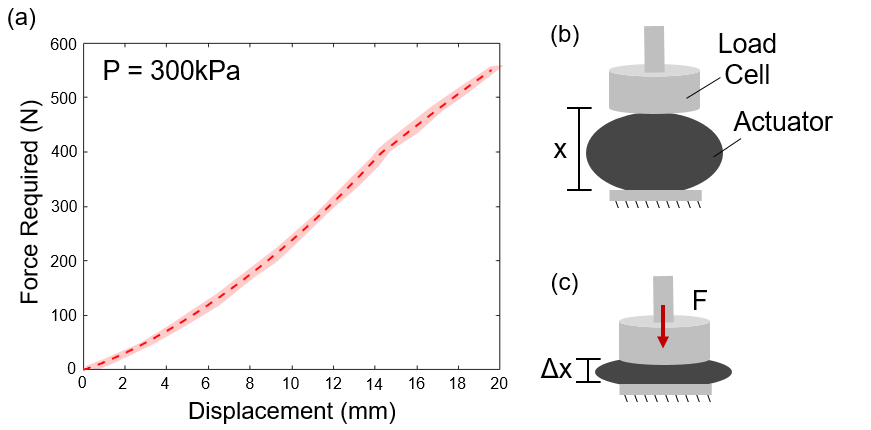
\includegraphics[width=0.3\textwidth]{stiiffnesstest.PNG}
\caption{Testing of individual air bladder, with the total pushing force of a single actuator constrained at 8mm - the distance each bladder sits apart from adjacent bladders in the array of bladders in the flexion actuator.}
\label{fig:stifftest}
\end{figure}

\begin{figure}
\centering
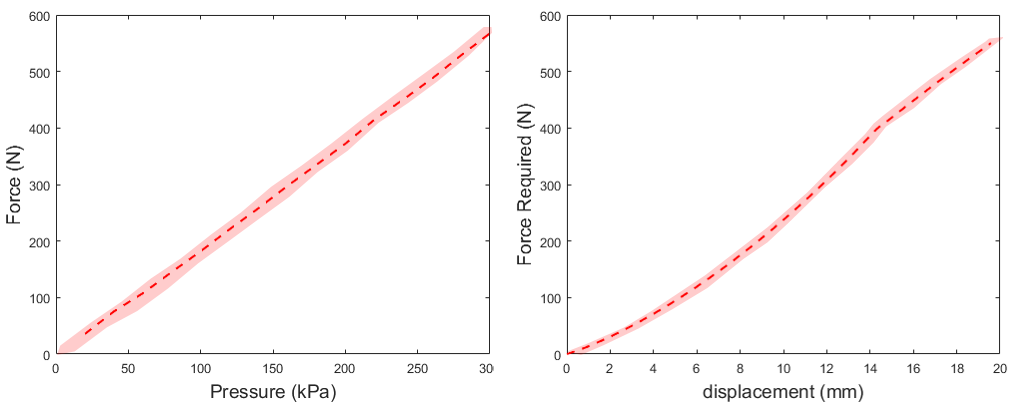
\includegraphics[width=0.5\textwidth]{singlebladder.PNG}
\caption{Test results in in the figure on the left show the resulting forces measured over a surface of a circle with a radius of 45mm.  The test results display the outcome of 5 iterations of  increasing the pressure in increments of 20 kPa.   Knowing the max forces the bladder was capable of, the bladder was then tested for stiffness at that same force (550N).
.}
\label{fig:stifftest}
\end{figure}

\subsection{Torque Test and Extension Implementation}

Due to the extremely high forces generated by a single actuator, the ends of the flexion actuator had to be constrained by a rigid structure, which served as a physical end-stop to mimic the boundary conditions set within the analytical torque models.  


\begin{figure}
\centering
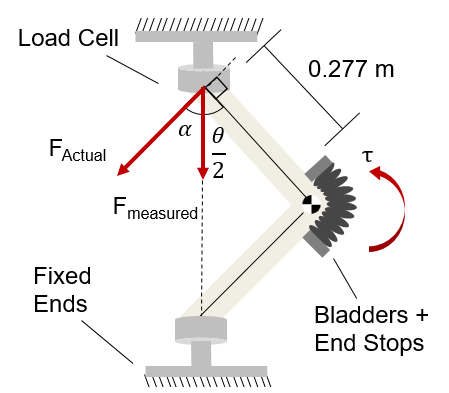
\includegraphics[width=0.5\textwidth]{torquetest.PNG}
\caption{Test setup for the torque measurements (left)}
\label{fig:stifftest}
\end{figure}

\begin{figure}
\centering
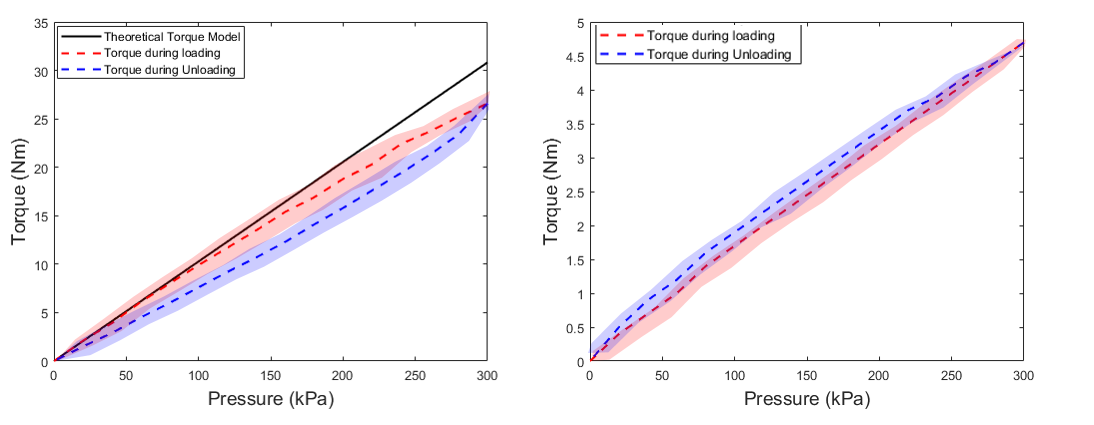
\includegraphics[width=0.5\textwidth]{torque.PNG}
\caption{Theoretical torque output of the device plotted against the actual test data (left), as well as the torque output of the extension bladders on the same testing apparatus (right).}
\label{fig:stifftest}
\end{figure}

The device was testing using a uniaxial tensile test machine.  The device was locked at a 90 degree bend in the elbow joint and fixed at both the top and bottom of the test arm as shown in Fig. X.  The flexion actuator was then inflated in increments of 20 kPa up to the maximum pressure of 300 kPa, at which point the device was predicted to reach its final torque output of 30Nm.  The device was loaded and unloaded to the the presence of any hysteresis, which wa minor but overall negligible as the system was able to reach a maximum of 27.6Nm of torque at 300 kPa, which is less than a 10\% error for the predicted 30Nm of torque.  The test was run for 5 iterations, resulting in a standard deviation of 0.67 for loading and 0.63 for unloading.  The extension actuators were also tested for the torque output and after 5 iterations the max torque was measured at 4.75Nm. 

\section{PARTICIPANT TESTING}

\subsection{Electromyography Device Testing of Exosuit}
The exosuit was tested on an able-bodied participant for a total of three iterations.  The participant was asked to hold their arm at a 90 degree bend in the elbow for 5 seconds for each of the following tests - the worst-case angle for torque about the elbow joint and strain on the bicep.  An EMG sensor was placed on the participant’s bicep and a baseline was measured without the device with the arm at rest, as well as the maximum effort performed by the bicep while the elbow was held at 90 degrees to show a maximum voluntary contraction (MVC).  With the minimum and maximum effort exerted by the bicep were used to normalized the following tests and plot the results.   The first test was to verify that the device was able to provide assistance to the bicep in lifting the unloaded weight of the forearm.  The participant lifted and held the arm at 90 degrees at the elbow with no assistance from the exosuit and then with assistance.  This showed a X.X\% reduction in muscle activity for a lift with no load.  Next, a load of 25\% of the user’s maximum lifting capacity was held at a 90 degree bend in the elbow first without exosuit assistance and then with exosuit assistance.  A X.X\% reduction in muscle activity was observed.  Finally, a load of 40\% of the participant’s maximum lifting capacity was lifted and held at a 90 degree bend in the elbow with and without assistance.  A X.X\% reduction in muscle activity was measured for this weight.  


\subsection{Range of Motion Study}
In order to verify that the device was not restrictive to normal human motion, a range of motion (ROM) test was performed to quantify the angles the user’s arm was able to achieve before and after wearing the exosuit.   Additionally, and EMG sensors was placed on the bicep to measure the muscle activity through the entire range of motion test both with the exosuit and without.  A 3-Dimensional motion capture system was used to track the user’s movement through the motion of a single ‘curl’ from full elbow extension to full elbow flexion.  The motion trackers were placed in positions as shown in  figure X.  The user performed a single curl with no assistance from the exosuit.  The user was then asked to perform the same type of motion relying on device to perform the entire range of motion.  The total range of motion decreased only X.X degrees while wearing the device, however the muscle activity decreased 60\% of the original effort exerted to achieve almost the same range of motion.      

\begin{figure}
\centering
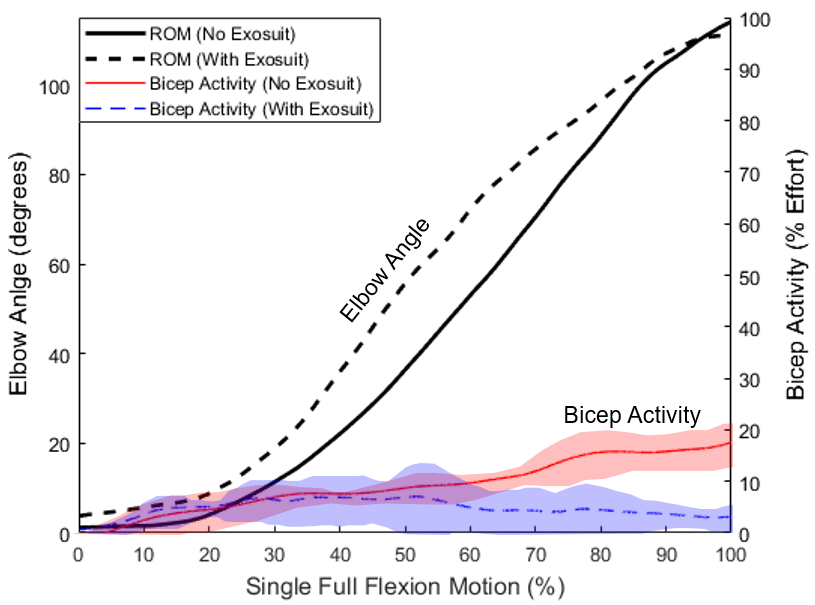
\includegraphics[width=0.5\textwidth]{ROM.PNG}
\caption{Theoretical torque output of the device plotted against the actual test data (left), as well as the torque output of the extension bladders on the same testing apparatus (right).}
\label{fig:stifftest}
\end{figure}

\section{CONCLUSIONS}

In this paper, the design, characterization, and evaluation of a lightweight soft robotic elbow exosuit was presented, aimed to assist in elbow flexion and extension of freight and warehouse workers. The design of the device was composed of two TPU actuator designed for the extension motion and an array of overlapping actuators enclosed in an inelastic fabric casing to assist the flexion motion. These actuators were tested and characterized for their force output on the experimental test setup.  From the results of the tests detail in section X, it was observed that the device was able to perform the primary task of providing 27Nm of torque about an elbow joint, within 10\% error the the predicted 30Nm chosen based off of the parameters chosen from the modeling of the system.  The design of the actuators allowed for extremely high force-to-weight ratios, providing a maximum stiffness of 28,200 N/m per actuator when inflated to 300 kPa.  

	It was found that some of the limitation of the device were related to how the higher-level forces were translated to the body.  While the device itself was able to produce 27Nm of torque, there were some issues regarding the ergonomics of the device when actually worn on the human body.  Because of the compliance of the human tissue and muscle,, the device became restrictive and uncomfortable  to the user when pushed to such high extremes, even when showing it was able to provide a reduction in muscles activity.  

The next steps for this device would be the implementation of user intent with EMG sensors to detect muscle activity and send signals to the corresponding actuators based on the needed motion for the users.  Another step would be to investigate a more mobile actuation system that could either be worn by the user in the field or run off of existing pneumatic systems.  With 70\% of the manufacturing industry having a major surplus in their pneumatic systems, devices such as the soft robotic elbow sleeve could be an efficient solution, not only to improve worker endurance and productivity, but also to utilize existing, untapped resources such as these pneumatic systems [20][21].  Adding force control and a closed-loop systems would be ideal for the final iteration of the device for real-world testing. 




\addtolength{\textheight}{-12cm}   % This command serves to balance the column lengths
                                  % on the last page of the document manually. It shortens
                                  % the textheight of the last page by a suitable amount.
                                  % This command does not take effect until the next page
                                  % so it should come on the page before the last. Make
                                  % sure that you do not shorten the textheight too much.

%%%%%%%%%%%%%%%%%%%%%%%%%%%%%%%%%%%%%%%%%%%%%%%%%%%%%%%%%%%%%%%%%%%%%%%%%%%%%%%%



%%%%%%%%%%%%%%%%%%%%%%%%%%%%%%%%%%%%%%%%%%%%%%%%%%%%%%%%%%%%%%%%%%%%%%%%%%%%%%%%



%%%%%%%%%%%%%%%%%%%%%%%%%%%%%%%%%%%%%%%%%%%%%%%%%%%%%%%%%%%%%%%%%%%%%%%%%%%%%%%%

\section*{ACKNOWLEDGMENT}

The preferred spelling of the word ÒacknowledgmentÓ in America is without an ÒeÓ after the ÒgÓ. Avoid the stilted expression, ÒOne of us (R. B. G.) thanks . . .Ó  Instead, try ÒR. B. G. thanksÓ. Put sponsor acknowledgments in the unnumbered footnote on the first page.



%%%%%%%%%%%%%%%%%%%%%%%%%%%%%%%%%%%%%%%%%%%%%%%%%%%%%%%%%%%%%%%%%%%%%%%%%%%%%%%%

References are important to the reader; therefore, each citation must be complete and correct. If at all possible, references should be commonly available publications.

% ********************************** Bibliography ******************************

\bibliographystyle{plain}
%\bibliographystyle{plainnat} % use this to have URLs listed in References
% \cleardoublepage
\bibliography{library} % Path to your References.bib file



% \begin{thebibliography}{99}

% \bibitem{c1} G. O. Young, ÒSynthetic structure of industrial plastics (Book style with paper title and editor),Ó 	in Plastics, 2nd ed. vol. 3, J. Peters, Ed.  New York: McGraw-Hill, 1964, pp. 15Ð64.
% \bibitem{c2} W.-K. Chen, Linear Networks and Systems (Book style).	Belmont, CA: Wadsworth, 1993, pp. 123Ð135.
% \bibitem{c3} H. Poor, An Introduction to Signal Detection and Estimation.   New York: Springer-Verlag, 1985, ch. 4.
% \bibitem{c4} B. Smith, ÒAn approach to graphs of linear forms (Unpublished work style),Ó unpublished.
% \bibitem{c5} E. H. Miller, ÒA note on reflector arrays (Periodical styleÑAccepted for publication),Ó IEEE Trans. Antennas Propagat., to be publised.
% \bibitem{c6} J. Wang, ÒFundamentals of erbium-doped fiber amplifiers arrays (Periodical styleÑSubmitted for publication),Ó IEEE J. Quantum Electron., submitted for publication.
% \bibitem{c7} C. J. Kaufman, Rocky Mountain Research Lab., Boulder, CO, private communication, May 1995.
% \bibitem{c8} Y. Yorozu, M. Hirano, K. Oka, and Y. Tagawa, ÒElectron spectroscopy studies on magneto-optical media and plastic substrate interfaces(Translation Journals style),Ó IEEE Transl. J. Magn.Jpn., vol. 2, Aug. 1987, pp. 740Ð741 [Dig. 9th Annu. Conf. Magnetics Japan, 1982, p. 301].
% \bibitem{c9} M. Young, The Techincal Writers Handbook.  Mill Valley, CA: University Science, 1989.
% \bibitem{c10} J. U. Duncombe, ÒInfrared navigationÑPart I: An assessment of feasibility (Periodical style),Ó IEEE Trans. Electron Devices, vol. ED-11, pp. 34Ð39, Jan. 1959.
% \bibitem{c11} S. Chen, B. Mulgrew, and P. M. Grant, ÒA clustering technique for digital communications channel equalization using radial basis function networks,Ó IEEE Trans. Neural Networks, vol. 4, pp. 570Ð578, July 1993.
% \bibitem{c12} R. W. Lucky, ÒAutomatic equalization for digital communication,Ó Bell Syst. Tech. J., vol. 44, no. 4, pp. 547Ð588, Apr. 1965.
% \bibitem{c13} S. P. Bingulac, ÒOn the compatibility of adaptive controllers (Published Conference Proceedings style),Ó in Proc. 4th Annu. Allerton Conf. Circuits and Systems Theory, New York, 1994, pp. 8Ð16.
% \bibitem{c14} G. R. Faulhaber, ÒDesign of service systems with priority reservation,Ó in Conf. Rec. 1995 IEEE Int. Conf. Communications, pp. 3Ð8.
% \bibitem{c15} W. D. Doyle, ÒMagnetization reversal in films with biaxial anisotropy,Ó in 1987 Proc. INTERMAG Conf., pp. 2.2-1Ð2.2-6.
% \bibitem{c16} G. W. Juette and L. E. Zeffanella, ÒRadio noise currents n short sections on bundle conductors (Presented Conference Paper style),Ó presented at the IEEE Summer power Meeting, Dallas, TX, June 22Ð27, 1990, Paper 90 SM 690-0 PWRS.
% \bibitem{c17} J. G. Kreifeldt, ÒAn analysis of surface-detected EMG as an amplitude-modulated noise,Ó presented at the 1989 Int. Conf. Medicine and Biological Engineering, Chicago, IL.
% \bibitem{c18} J. Williams, ÒNarrow-band analyzer (Thesis or Dissertation style),Ó Ph.D. dissertation, Dept. Elect. Eng., Harvard Univ., Cambridge, MA, 1993. 
% \bibitem{c19} N. Kawasaki, ÒParametric study of thermal and chemical nonequilibrium nozzle flow,Ó M.S. thesis, Dept. Electron. Eng., Osaka Univ., Osaka, Japan, 1993.
% \bibitem{c20} J. P. Wilkinson, ÒNonlinear resonant circuit devices (Patent style),Ó U.S. Patent 3 624 12, July 16, 1990. 


% \end{thebibliography}




\end{document}
